\documentclass[10pt,twocolumn]{article}

% use the oxycomps style file
\usepackage{oxycomps}
\usepackage{hyperref}
\usepackage{graphicx}

% read references.bib for the bibtex data
\bibliography{references}

% include metadata in the generated pdf file
\pdfinfo{
    /Title (Comps Paper)
    /Author (Alec Phillips)
}

% set the title and author information
\title{Comps Paper}
\author{Alec Phillips}
\affiliation{Occidental College}
\email{aphillips2@oxy.edu}

\begin{document}

\maketitle

\section{Problem Context}

% come back to this section last and give all the context needed to understand the project and the following sections

Software testing is a core principle of computer science that is often overlooked or at least under-emphasized in 
computer science education. Testing is an integral part of any software project, and is a skill that must be developed 
like any other technique in software development. It takes considerable knowledge to be able to develop robust and 
efficient test cases that create confidence in one's code. Thus, this skill should be honed and developed along with 
other programming techniques. Software testing is also nuanced and there are numerous testing techniques that are 
important for students to learn about and have experience putting into practice. The importance of software testing 
serves as the motivation behind my comps project idea; I would like to create a web application that teahches software 
testing techniques and exposes introductory to intermediate level students to related concepts. 

A web application that teaches software testing would be beneficial to computer science education in general because 
it could be added to a standard computer science curriculum to help students get exposure to the concept. My goal is to 
provide comprehensive materials on software testing as well as hands on exercises where learners can put the concepts 
into practice. Instructors could add this to their curricula, or self-learners could utilize it to gain exposure to 
software testing techniques. 

\section{Technical Background}

This section will cover the relevant terminology that is critical for understanding the technical side of my project as
well as the general goals of my application. These include general software testing techniques, as well as related topics
such as test-driven development, error handling, edge case identification, and debugging. It is important that students
view testing as an important aspect of software development.

\subsection{Software Testing Techniques}

\subsubsection{Scopes of Testing}

Testing is a nuanced aspect of software development, and there are several key techniques that are commonly employed for 
writing tests. These different techniques are often used together to comprehensively exercise code, as they work 
together to test a single application in different ways. Thus, it is not sufficient to know just one of these 
techniques; a competent developer should be familiar with all of them, in order to know what to utilize depending on 
their needs. Software testing can be broken up into four main categories depending on the scope and motivation of the 
test. These categories are unit testing, integration testing, end-to-end testing, and acceptance testing 
\cite{Luo2001Article}. These are the four categories of testing that I plan to teach in my application, so it is 
important to elaborate on them in this section. 

\begin{itemize}
    \item{Unit tests are those that have the narrowest 
    scope. These are tests that apply to individual modules of code. Defining a specific unit of the code is up to the 
    developer, but it is standard for unit tests to apply to specific functions, although it can also apply to an entire 
    module.}
    \item{Integration testing checks that the individual units are interacting as expected. This means that the interfaces 
    between the units as well as the general information flow between them should be exercised.}
    \item{System, or end-to-end 
    testing evaluates the overall requirements of the entire application. System tests would generally involve providing 
    inputs at the most general or external level, and evaluating that the outputs are as expected. For these tests to pass, 
    all the internal processes of the aspect being tested must be functioning correctly.}
    \item{Acceptance testing is the final 
    step, in which it is determined if the piece of software conforms to the general specification requirements, and also 
    aligns with what the client or user is expecting \cite{Luo2001Article}. }
\end{itemize}
   
\subsubsection{Styles of Testing}

In addition to the four categories of testing discussed above, there are also two styles of tests that serve different 
purposes, and can each be applied to a either subset or all of the above categories. Once again, it is important to know 
both of these styles, as a thorough test suite should incorporate both. These two types are functional and structural 
testing. Functional is the more broad of the two, in the sense that any of the four categories of tests above can be 
functional in nature. Functional tests are also called 'black box' tests. These tests are ones that assume no knowledge 
of the underlying implementation of the code being tested, and only examine the expectied behavior of the section of 
code being run. These are tests that could be written provided only with the API for a class, or the definition of a 
function, along with an understanding of the expected output. In contrast, structural tests, or 'white box' tests, 
take into account the implementation of the code. They are geared towards exercising specific sections of the 
implementation to make sure that the internal code is operating as expected. This is looking deeper than just expected 
outputs, but instead at the operations taking place within the code. Unit tests, integration tests, and system tests 
can all be structural, however acceptance tests cannot. This is because acceptance tests evaluate whether the system's 
bahavior aligns with what the end user is expecting, and the user or client will (likely) not have any understanding of 
the internal implementation of the code \cite{Sawant2012Article}.

\subsubsection{Arrange, Act, Assert}

Along with these types/styles of testing, my application includes information on testing best practices. These include
the \textit{arrange}, \textit{act}, \textit{assert} style of writing tests. This is the generally accepted format of 
structuring each test case. 
\begin{enumerate}
    \item{The arrange step involves setting up any context necessary to run the test - this could 
    include initializing objects and variables that will be involved in the test.}
    \item{In the act step, function calls are made that exercise the behavior under test. Results of these calls are set
    to variables.}
    \item{The variables resulting from the act step are then checked for correctness in the assert step. This involves
    some form of \textit{assertion} statement that will see if the act step resulted in the expected values and throw
    an error if the result is not as expected.}
\end{enumerate}

\subsubsection{Error Handling}

Finally, the application exposes students to the concept of error handling in code. This is more tangentially related to 
testing but is still important to understand. It relates to software testing because the appropriate use of error handling 
makes code easier to test and debug. My application focuses on error handling to the extent of including a content section
that goes into detail on how to raise errors in javascript, how to catch and handle these errors, as well as how to test
for errors being raised. It can be easily overlooked that test cases can be dedicated to checking for a particular type 
of error being raised in a certain situation, so it is important and relevant for students to learn about how to test 
for raised errors in this way. 

\subsection{Test-Driven Development}

Initially, I had wanted my application to specifically have students practice the process of test-driven development. 
However, after beginning to develop coding exercises, it became clear that it is difficult to have users practice this 
development strategy within the confines of an application. This is because the process of test-driven development inverts
the standard order of writing and then testing code, and can be abstract. I decided that it would be more engaging for students to be able to 
immediately run their test cases against a specific function. Thus, I did not include exercises specifically on test-driven
development, but it is still explained in the Learn section of my application. Because TDD is increasingly being used in 
industry, students should have an understanding of the general process. 

It is important to understand that test-driven development is not a testing strategy, such as 
the ones discussed in the prior section. Instead, it is a software development framework, meaning
that it informs the entire software development process, not just the testing aspect \cite{George2004Article}.

Test-driven development fits within the Agile approach of software development \cite{Janzen2005Article}. Agile 
strategies tend to involve an iterative process that repeats until a project is complete, and is a common industry 
practice. This sits in contrast to older styles of development, such as Waterfall, which have more upfront design 
prior to coding. Test-driven development is also considered a practice of extreme 
programming, or XP, which takes basic development principles, such as testing, and emphasizes them to drive the entire 
development process \cite{Desai2008Article}.

Test-driven development lays out a detailed approach to developing software that is centered around allowing 
code testing to push forward the project, in the sense that test cases are written that in turn motivate the code 
that needs to be written. 

\subsubsection*{Steps of TDD:}
\begin{enumerate}
    \item write test cases for the next unit of code being added to the project
    \item write the code that the first test case is exercising (until it satisfies the test case)
    \item refactor the code as needed (both function and test case)
    \item re-run all existing test cases to check for regressions in the code base \cite{Bhat2006Article}
\end{enumerate}
This process then repeats until the project is complete. Thus, this process informs the 
development of the entire project, not just the testing aspect. 

 
% TODO:
%   Can't talk about this unless I add to the TDD section of the Learn area to talk about some of the downsides/limitations
%   of TDD

% It is also important to acknowledge that there are downsides to test-driven development. These shortcomings are valuable 
% for me to understand before incorporating test-driven 
% development as an main aspect of what my application will teach, as well as for users to understand. I do not want to 
% present the concept as the ultimate or only way to approach software development, however I believe it is useful for 
% students to be exposed to the concept and that it a valuable way for students to learn the importance of software testing. The main 
% limitations of test-driven development stem from the fact that there is little emphasis on overall system design 
% \cite{George2004Article}. This can necessitate heavy code refactoring later on, since everything is developed in small 
% chunks. Thus, it is important that my application conveys the importance of overall system design so that students are 
% aware of its importance. I want users of my application to be aware of these considerations, should they choose to practice test-driven 
% development in their own projects. 

\section{Prior Work}

This section explores some of the literature on incorporating software testing in to computer science education, as well 
as some of the areas that this can be improved. This research helped guide and motivate my project in terms of helping me 
determine what my application should focus on and the gaps that it is helping to fill.

% TODO:
%   same as below, this can be discussed IF I improve the Learn section on TDD

% This section will also briefly look at some research into the effectiveness of test-drivenuse these to get a better sense of the 
% concept and its efficacy. 

\subsection{Software Testing in Education} 

% TODO:
%   this whole section needs to be re-framed to focus less on TDD and more on just learning testing...

This section will discuss some of the strategies that have been used to teach software testing and test-driven 
development in the past. This will inform the approach that I take for teaching software testing in my application. 
I came across a significant amount of discussion on the reasons why software testing is undertaught, as well as why 
students find it to be an uninteresting concept to learn. Additionally, there was discussion of how test-driven 
development specifically could be integrated into computer science education. 

The lack of emphasis on software testing in education stems from both students and instructors. Computer science courses 
as well as entire programs are already packed with material, so adding lessons or assignments focused solely on testing 
can be infeasible \cite{Edwards2003Article2}. Additionally, students often find implementation of projects more exciting 
than testing their code, and testing can often appear tedious. Students can also be unmotivated to 
test their code, because they do not want to see it fail \cite{Carrington1997Article}. This is also something that I 
have noticed as a teaching assistant; students will sometimes write test cases that are very specific to their code, 
when more general test cases would not pass. From being a TA I have also noticed that, in general, students do not take 
writing test cases very seriously. Even when instructed to write tests, students in Data Structures will treat it as an 
afterthought, heavily prioritizing other aspects of their projects. 

If the incentives were flipped, and students had 
more of a desire to write failing test cases, they would likely take the task more seriously. This can inform the way 
that I design my practice exercises in the application; instead of having students write code and then test it, I would 
provide them with code that they then need to exercise with test cases, and their performance on this activity will be 
dictated by how robust their tests are. One potential way this could work is by providing a function that fails on some 
edge case which the learner has to identify on their own and then write a test that causes the provided code to fail. 
This would incentivise the student to thoroughly understand both the goal of the function, as well as the actual code, 
and would provide the desire to write a good test that fails the code. 

There is also existing research on having students apply the concepts of test-driven development in order to learn 
computer science in general. This would make software testing a more integral part of every project that students take 
on, shaping the belief that testing is an important part of writing code. Some strategies for implementing this in an 
education setting were to make students fully responsible for demonstrating the correctness of their code 
\cite{Edwards2003Article1}. This would mean that students would not be given any automated test results before 
submitting their code, and would instead be responsible for determining their code's correctness on their own. This may 
be unrealistic to implement in a classroom setting, because it would likely put an even greater strain on students, 
espcially when computer science classes are already time consuming and challenging. However, I can base the exercises in 
my application around this idea, requiring students to write code along with test cases that must reach a certain amount 
of coverage of their code, or catch certain edge cases. 

% TODO:
%   don't add this until the section in the application on TDD is improved
%   this section is not currently very relevant to my application...

% \subsection{Test-Driven Development in Industry}

% I looked at two studies exploring the effectivenss of test-driven devlopment in industry. Both of these compared a group 
% that used test-driven development and a control group that employed their standard development practices. The first 
% study looked at two divisions in Microsoft (Windows and MSN). This study looked at effects of test-driven development on 
% code quality as well as total development time. Code quality was calculated by number of code defects as well as 
% KLOC (thousands of lines of code) between teams using test-driven development and teams in the control group. 
% Using these metrics, the study found that, for both departments, code quality was higher with test-driven development, 
% while development time was also higher; the Windows division had 2.6 times higher code quality and the MSN team had 4.2 
% times higher code quality using test-driven development, but also experienced 35 and 15 percent increases in development 
% time respectively \cite{Bhat2006Article}. It is encouraging that the implementation of test-driven development increased 
% code quality, and interesting that it also raised development times. The reason behind this could just be that the 
% developers were more accostomed to the workflows of their previous development strategy, so they were slightly slower 
% when using test-driven development. However, this difference in efficiency is fairly significant, so it is worth 
% considering the balance between code quality and work efficiency. 

% The second study took programmers from three companies and had them pair program a bowling game. The programmers were 
% split into test-driven development groups and control groups. They were evaluated on their ability to pass a set of test 
% cases that they were not allowed to test against before submitting, and also their ability to write their own comprehensive test cases. 
% Their time spent to complete the project was also assessed. This study found quite similar results; the test-driven 
% development groups passed more of the test cases, but took longer to develop the project by 16 percent 
% \cite{George2004Article}. This aligns with the findings in the previous study, and it is interesting that once again the 
% test-driven development groups took longer to develop the project than the control groups. However, it is positive that
% in both studies, the use of test-driven development seemed to lead to fewer errors. Another interesting finding from this 
% study is that all but one of the control groups failed to provide comprehensive test cases for their code, despite being 
% directed to do so \cite{George2004Article}. I find this to be particularly interesting, because even professional 
% developers chose not to thoroughly test their code when it was not built in as a part of their development process. This 
% emphasizes the value of test-driven development's integration of testing into the coding process, because even 
% professionals are not always inclined to thoroughly test their code. 

\section{Ethical Considerations}

An application geared towards education may initially appear to be ethical, however there are still potential moral issues. 
Any application or product geared towards 
users and has the potential to affect real world outcomes has the inherent possibility of affecting negative change. 
Additionally, there are a number of ethical concerns that arise from taking on the role of educator; for instance: what 
are the ethical and pedagogical obligations that an educator has to the students? There is the also the topic of power, as this 
application’s service will likely only affect those who already have 
access to computer science education, reinforcing the current power dynamics in terms of who has access to education and 
the ability to learn computer science. Additionally, it reinforces power dynamics existing around who has internet 
access. Finally, there is the concern of security, as any web application is open to possible attacks, and any service 
that stores user information, as mine likely will, must consider the risk of exposing individuals’ information that they 
have entrusted to you and the service. Despite the initially benign appearance of this project, these ethical 
considerations emphasize that there are still potential ethical issues present that need to be considered carefully. 

\subsection{Educator Obligations}

Taking on the role of educator places one under an ethical burden, as they are entrusted to have expertise on 
the topic and the ability to adequately convey accurate information. The University of Michigan education department 
offers a simple overview of nine core ethical obligations that teachers should uphold. Several of the obligations that 
they bring up will be difficult for me to uphold within the context of this project, specifically
personal responsibility and competence. 

The webpage defines personal responsibility as taking “responsibility for obstacles to student success and to work 
assiduously to ensure equitable access to learning opportunities” \cite{MichiganEducation}. This poses an issue for 
my project because of the amount of time I will be able to dedicate to maintaining this project after it is completed 
and the impersonal nature of an educational application. If this application ends up actually getting deployed, it would 
be infeasible for me to be responsive to every user and their individual needs. 

The article defines competence as “[developing] and continually [working] to improve instructional competence, and to 
strive to engage in professionally-justified teaching practice at all times” \cite{MichiganEducation}. This is 
similarly infeasible because of the commitment that it would take to actively continue improving my instructional 
competence. Within the context of my project, it would require continued updating of the materials and content, as well 
as continuing to further my knowledge to better serve the users of the application, which are not responsibilities that 
I can confidently commit to at this time. These two examples represent the issues that come along with taking on the 
role of educator and building an educational site. In order to address this, it is important that, if this application 
is to be deployed, I only allow it to be active for as long as I can uphold these obligations. 

\subsection{Power Reinforcement}

In addition to the general ethical issues of building an education based application, there is the problem of who will 
have access to this application, and how that reinforces existing power dynamics in the world of computer science and 
technology. Power and computer science are tightly intertwined; technology is nearly omnipresent in our world, and many 
of the most influential and powerful individuals are those who control large technology companies. One clear factor that 
differentiates power in computer science and technology is whether or not someone has 
access to the internet. Individuals who have easy access to the internet are much more easily able to interact with 
existing technologies and web applications, and also have much more access to learning how to interact with computers in 
general. The issue with this web application, and conveying educational material over the internet in general, is that 
it is only making information more accessible to those who can already easily access it. Even if my application makes 
the information easier to learn 
or more enjoyable, it is not reaching a new audience or further distributing access to learning computer science. This 
then reinforces the existing power structures that exist in computer science. 

There is already a large power difference between those who have access to the internet 
and those who do not. The more effective my application is, the more I would be contributing to that power difference. 
The power differences caused by unequal internet access have been well documented, and play a role in global power 
dynamics as well. The advent of the internet has created easy access to information and communication, however this only 
applies to those who have access to it. Societies that do not have the luxury of widespread internet access do not get 
these same benefits, which increases the power differentials between these societies \cite{Fang2018Article}. This 
emphasizes the importance of the relationship between internet access and power. Therefore, further empowering those 
with internet access by means of a web application that only those individuals can benefit from will inherently further 
these existing power dynamics.

Power differences as a result of internet access habe been further exacerbated by the COVID-19 pandemic. This has been a 
prevalent issue in the academic sphere; students 
who have access to reliable internet can more easily and consistently access their courses, and do not have to worry 
about missing material because of something outside of their control like stable internet \cite{Lai2020Article}. 
This emphasizes that, currently, those without internet access are experiencing even greater challenges as a result of 
the pandemic, so introducing more web based applications will further this divide. These issues are important to 
consider, but my hope is that ultimately my application can provide more benefit to individuals and make computer 
science more accesible overall. 

\subsection{Ethics of Security}

This application also brings in the issue of security. The application will likely store user data, such as passwords 
and usernames in a database. If the application is attacked, this user data could be leaked. Additionally, a part of my 
application involves running users' code to evaluate their performance on coding exercises. This brings in the 
possibility of malicious code injection. To ensure that it is ethical to deploy this application, it will be critical 
for me to make sure that I am diligent in securing the 
application from potential attacks such as these, in order to feel confident that my application is not putting anyone's 
information in danger. 

\section{Methods} 

% for the actual comps final paper:
%   - the methods will talk more about the iterative process of testing the app, getting feedback, and then 
%     implementing that into the project
%   - can also include some of the stuff about code design, UI justification, and diagrams of UI webpage/route flow
%   - less stuff about actual code design, especially for server-side & database (this will go on code documentation)

% for the comps proposal paper:
%   - add section at the beginning justifying my UI design
%   - add diagram of UI flow (pages/routing)
%   - add discussion of design specific to test-driven development
%       - how I plan to design exercises to teach this concept (just writing tests, writing code & tests, etc.)
%   - brainstorming of how I could go about the iteration of testing and improving the app
%       - how will I test, what sorts of things would I ask testers

\subsection{Implementation}

The project is build fully using React.js and javascript, along with CSS and HTML. Originally, I intended to have a server-side 
API running that would process code submissions, as well as a database to store the excercises as well as user progress. This 
would require the application to have a login page, and the code evaluation would need to involve using subprocesses or something 
analogous in order to asynchronously run users' code submissions. Additionally, running user generated code on the server-side 
is inherently dangerous, because they gain access to the file system and OS of the server. In order to safely run their code,
I would have needed to either restrict what the user is allowed to write in the code editor, or heavily verify their submissions. 
This would be very difficult and time consuming to do sufficiently, and would take away from the ability to focus on other aspects 
of the application like usability. 

All of these factors lead me to end up choosing to build the application as a server-less web-page. This way, the user generated 
code is only running in their web-browser, and so they have no ability to break a remote server with their code. Additionally, 
this takes away the reliance on having a network connection to submit code, and there is no need to handle multiple submissions 
asynchronously, as would be necessary if a back-end were implemented. This also makes the application very fast, since it is 
independent of the speed of the network. One drawback of this design is that all coding exercises had to be in javascript, 
because that is the only language that can run in the web-browser, without the use of some sort of cross-compiler that would 
convert from another language into javascript. I had initially wanted to have the exercises be in python, however javascript 
is also a good language for students to get introduced to, especially if they are interested in going into front-end development. 

% TODO:
%   talk about how I got around not having a db, how I store user progress, etc. 
One main drawback that the serverless design posed was the lack of a database. My main concern without a database was figuring
out how to store the content descriptions and exercises, as well as storing user progress. However, I realized that another 
way to achieve the storing of user progress was through the browser's localStorage feature. This is a structure stored by the 
browser that each webpage can access through a simple get/set API. I leveraged this to store a list of exerciseIds corresponding 
to the exercises that the user has completed. Upon a correct exercise submission, the application updates this list, which is 
saved and loaded on subsequent visits to the application. In order to get around storing other data that would have been put 
into a database, I stored the data in javascript objects. This simulates the way that the data would be stored in a non-relational
database. I looked into serverless database options, but after learning that the localStorage option was available, I chose to go 
down that route because it seemed more feasible for the scale of the application. 

Additionally, the lack of a server came along with several advantages for usability as well as ease of development. The general
usability is improved because the lack of a back-end system means that the application is very quick and responsive, because 
there is no reliance on network connection speeds in sending information back and forth. Additionally, since all the data 
that the application needs in order to run is held in the browser upon initial loading, if network connection is subsequently 
lost, the application is still fully usable. This is advantageous because it makes the application more usable for individuals 
with less stable internet connections. In terms of ease of development, the lack of a server-side made the application much 
easier to deploy; I was able to deploy through github pages, which was a very simple process. This ease of deployment made 
it easier to have an initial deployment out earlier, meaning I was able to do a first round of user evaluations fairly early, 
allowing me more time to iterate on feedback and get input from users. 


\subsection{Interface Design}

My main motivation with the interface was to have a simple but still visually appealing design, focusing more on having 
a very intuitive page layout. My general design was inspired by \href{https://codingbat.com/java}{CodingBat}, which is one 
of my favorite online computer science education resources \cite{CodingBat}. This cite was created by a Stanford professor 
for his introductory computer science students. I find the overall experience of using the 
website to be intuitive and simple. The user interface is bare-bones and easy to navigate.

One difference that I wanted for my application was to have a more clear path through the material so that the content can
build on itself. I wanted this for my application because I want the user to be working through the exercises in order so 
that they can draw on topics introduced earlier on in order to solve later problems. Additionally, since it is intended to 
be a first exploration of software testing as well as the javascript language, I believe that it makes sense for users to 
work through the problems from the beginning. In order to enforce this, I added the feature of unlocking exercises; at 
the beginning, the first exercise of each section is unlocked, and subsequent exercises become unlocked as the user 
completes the problems. I also believe that this makes the application more fun, because it gamify the user experience. 


% This figure is no longer relevant, but could choose to include a different UI diagram...

% figure \ref{UI-flow-diagram}.
% \begin{figure}[!ht]
%     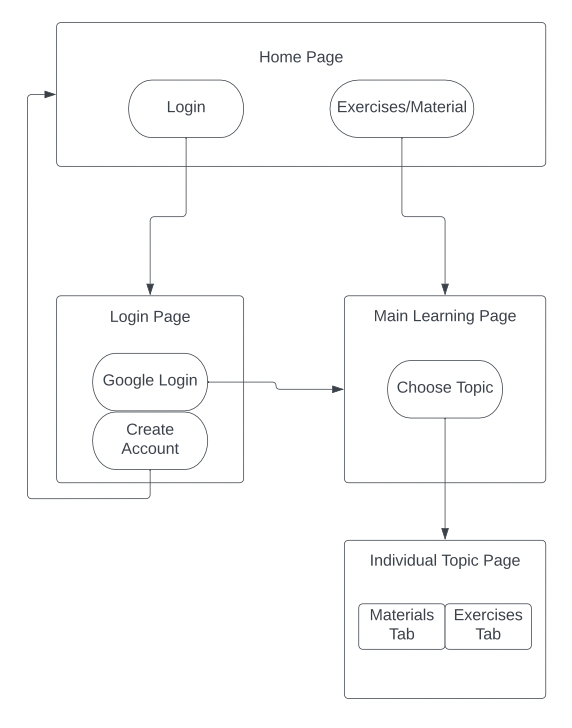
\includegraphics[scale=.7]{./images/UI-Flow-Diagram}
%     \caption{Intended Application UI/Page Flow}
%     \label{UI-flow-diagram}
% \end{figure}


\subsection{Content Design} 
% TODO:
%   here, justify the design of the content, specifically the way the Learn materials are presented, as well as the 
%   decision to include both edge case & debugging exercises (to give an entry point into learning javascript and reasoning abt correctness)
%   talk about the process of designing exercises
%   connect to the previous section on Hands on Research
%   etc. 

As an educational application, a critical piece of my project was designing the content and programming exercises.
I made sure to talk to many individuals about what would be most helpful to include and focus on in the application.
The main takeaways were that it is important to include hands-on exercises as well as detailed 
examples, as opposed to simply having descriptions on types of testing. However, it was also emphasized that the materials should be concise to avoid being overwhelming. This was important 
to me as well, because I want this to be a concise but useful introduction to the nuances and types of software testing. 
One helpful piece of advice that I recieved on designing the exercises was to focus on common errors, such as off by one 
and improper input formats. By focusing on commonly occuring errors, users of the application will be able to gain 
familiarity with some of these and be better prepared to avoid them in the future. 

In terms of the specific types of exercises included in the application, I had initially wanted to focus on implementing 
a combination of unit and system-style testing exercises. However, some aspects of development that I had overlooked took 
more time than expected, and I ended up focusing more on including a combination of edge-case identification and unit testing 
exercises, with minimal system test exercises. This ended up being more feasible within the time constraints of the semester. 
However, I believe that the application still holds value as a teaching tool or for general student use. The edge-case 
identification exercises are still beneficial because it teaches students to reason about code correctness and consider 
the range of possible inputs and deeply understand the code presented. Additionally, these exercises prompt users to both 
identify an input that causes a function to break, and then actually debug the code. This is useful for gaining a deeper 
ability to reason about code, and offers an entry point into learning javascript for the user. 

The test-writing exercises involve writing test cases that use assertion statements, with the goal of maximizing branch 
coverage on a given function. In the initial warm-up problems, the code being tested is provided, so the user can step 
through the function and more easily determine what inputs to provide to fully cover the branches. However, in subsequent 
exercises, a description of the behavior of the function is provided, but the actual code is obscured. This forces the 
user to consider how the function would be implemented in terms of the necessary control flow. To aid the user in this 
task, on a given submission attempt, they are given feedback on the percentage of branches that their code covered, as 
well as whether any of their assertion statements failed.

I ended up implementing one system-level test exercise, which involves the user writing a series of assertion tests on a
larger scale API. This exercise is the most difficult of all the content and is only unlocked after a user has completed 
all the unit test exercises. This way they have the proper context to be able to complete the system test exercise. This
exercise involves the user writing test cases against a mock course registration system. They are provided with the documentation 
for a CourseScheduler class with its member method stubs. Additionally, they are given the starting state of a 'database' 
which is actually implemented as a series of javacsript objects. However, this simulates the experience of writing code 
that interacts with a back-end database. For this exercise, users are also trying to raise the overall branch coverage, 
and to do so must interact with all the methods in the CourseScheduler class and reason about what combinations of 
interactions will cause certain operations to occur. For instance, students need to exercise a prerequisite-checking function,
but to do so they must enroll students in courses, increment the semester (so that students have then completed prerequisite 
courses), and then enroll the students in courses they are now qualified for. 


\subsection{Iterative Project Improvement}

Since I was able to deploy an early version of the project, I had time to do two rounds of user evaluations, allowing me 
to make iterative improvements to my project based on user feedback. In my first round of feedback, I used a survey that 
gauged the quality of the teaching content, the clarity of the exercise directions, the difficulty of several of the 
exercises, as well as overall user experience. From this first round of evaluations, I learned that the directions for 
the exercises could be made more clear, and that it would be helpful to include hints for some of the more difficult 
exercises. Additionally, it was noted that the feedback on coding exercises could be more detailed so that the user 
has more of a sense of what they did wrong. After this feedback, I added a hint area for each exercise, and improved the 
feedback reporting area to be more clear and visually appealing. 

In addition to using a survey, I watched individuals interact with the application to get a sense of how clear it is to 
use and where individuals get confused. One main takeaway from this was that users sometimes found it difficult to know 
where to start with the coding exercises. The exercises are displayed in rows, and I intended for them to be attempted 
from top-left to bottom-right. However, I noticed that this was not always intuitive, and this informed my decision to 
add the feature of locking/unlocking exercises as the user progresses. This enforces the order and provides a clear visual
of where to start. 

This type of interactive testing also exposed some bugs in the code evaluation system, specifically with the system test
exercise. One more advanced student tested the exercise and noticed that one specific series of interactions caused the 
exercise to break, so I was able to identify and fix the bug. Additionally, users identified multiple spelling errors in 
the application. 


\section{Evaluation}

To formally evaluate my project, I chose to focus on three main criteria:

\begin{enumerate}
    \item Teaching Quality (of written teaching content)
    \item Exercise Quality (clarity of directions, difficulty)
    \item Overall Learning Outcomes
\end{enumerate}

As discussed above, these were evaluated in two stages, first one a larger scale with a survey that was sent out to 
members of the computer science community, and secondly with one on one user interviews where interactions with the 
application were observed. 

\subsection{Round 1 - User Survey}

\subsubsection{Survey Design}

The survey was designed to target the three areas above for testing. Specifically, users were prompted to:

\begin{itemize}
    \item read the content on unit testing
    \item read the descriptions of three exercises (one edge case identification, one debugging, one unit testing)
    \item attempt to complete the three problems within two to three minutes
\end{itemize}

This allowed me to gain a sense of how effective each of the evaluation criteria were met in an early version of the project.
At this point in the implementation there were not yet system test exercises, so this aspect could not be evaluated. The 
problems that users were asked to complete were the rainfall problem for edge case and unit testing, and a fizzbuzz 
variation with an off by one error for debugging. 

\subsubsection{Participation}

The survey was sent to ten upper division computer science students (students either majoring or minoring in computer science
who have participated in an upper division course), as well as one section of twenty-eight introductory computer science students.
Seven of the upper division students participated in the survey, and no introductory students participated. This was problematic 
because my application was intended to be geared specifically toward introductory students. However, the findings actually 
indicated that the more advanced students could still benefit from using the application, which makes me believe that a wider 
target audience could be appropriate.

\subsubsection{Results}

For the category of teaching quality, students indicated that, their 
prior knowledge of unit testing was ~2.14 on a scale from one to five. After reading the learn section on unit testing, 
respondents rated their understanding at a 4 on the same one to five scale. Additionally, they rated the clarity of the 
section as ~4.57 out of five. This was a satisfactory outcome, indicating that even for more advanced students, they felt 
that the section taught them something new. This is especially telling because the section they read was on unit testing, 
which I would have assumed to be the type of testing that advanced students would be most familiar with, however they still
indicated positive learning outcomes. 

For evaluating the exercise quality, students indicated the clarity of the exercise descriptions as well as whether they 
were able to solve the problem for
each of the three types of problems that they attempted. Repondents reported average clarities of ~3.86, 4, and ~4.23 out 
of five for the edge case, debugging, and unit testing exercise directions respectively. These ratings indicate that users 
were generally able to determine what was expected for each type of exercise. However, in the written feedback area, some 
users indicated that the input format for edge case problems could be made more clear. In terms of difficulty, the solve 
rates were 71.43\% (edge case), 85.71\% (debugging), and 42.86\% (unit test). These were all problems that I would have 
rated as easy to medium in terms of the problems that could have been chosen. Additionally, respondents were asked to only 
spend up to three minutes solving the problems. These results indicate that students had the most trouble solving the 
unit testing exercise within the time limit, which reinforces the general idea that students would benefit from such 
exercises/practice. However, this gave me a good baseline for understanding how my perception of problem difficulties 
translates to users' experiences.

In terms of overall learning outcomes, it becomes clear from the findings above that students seem to benefit from interacting 
with the application. This is emphasized by the fact that even upper division students felt that they gained knowledge from 
the written materials, and also were not able to easily complete the unit testing exercise on the rainfall problem. Additionally,
on a Likert scale from one to five, when asked if they would liked this application to have been incorporated into their 
introductory computer science course:

\begin{itemize}
    \item 14.29\% gave a rating of 3
    \item 57.14\% gave a rating of 4
    \item 28.57\% gave a rating of 5
\end{itemize}

Overall the sentiment was positive and indicates that students would generally like to see this incorporated into their 
curriculum. Additionally, 100\% of respondents indicated that they felt that they learned something through interacting 
with the application. 

Despite the limited engagement with the survey, especially from introductory students, the findings were informative in 
providing a baseline of the applications effectiveness in relation to the three main evaluation criteria.



% for final comps paper (could also do this in this paper too):
%   - discussion of evaluation metrics could actually go before the methods, since it will be useful context since they
%     will get discussed in the methods (how evaluation helped me iteratively improve the project)

% for comps proposal paper:
%   - consider putting eval section before methods
%   - more specific about how i will survey users 
%       - how/where will I get people
%       - what i will have them do
%           - possibly have some who used the app and some who didn't both answer questions & take a short test
%               - could have them write test cases, or reasoning questions about edge cases, etc.

% \subsection{Usability}

% As opposed to the robustness testing, the user experience  of the application will 
% require user-testing. I would like to get at least ten respondents who are computer science majors at Occidental College 
% to evaluate this aspect of the project. It is important that they are computer science students, because I will be 
% having them evaluate the text editor, and I would like them to have a frame of reference going into this part of the 
% evaluation. I will create a Google Form survey that asks respondents to evaluate how 
% intuitive and usable the application is. There would be several prompts for the users in order to give them experience using the applicaion 
% before responding to the survey questions. First I would prompt them to spend two minutes exploring the application 
% freely to get a feel for the organization. Then I would prompt them to navigate to a specific exercise on the website, 
% in order for them to assess the difficulty of getting to a particular page they want to get to. This way, they would 
% get to see the entire UI flow and see all the pages. Finally, I would ask 
% them to try typing into the code editor. The survey questions would have them rank: 1 - their overall impression of how 
% intuitive the application layout is, 2 - the difficulty of finding the particular webpage that they were directed to 
% find, 3 - the organization of the educational content, 4 - the design of the exercise/material pages, 5 - the visual 
% appearance of the text editor (text highlighting and language accuracy), 6 - the experience of 
% typing in the editor in terms of responsiveness. Each of these would be ranked on a Likert Scale from 1 to 5. 
% Additionally, I would offer an open ended feedback section at the end. This would be valuable during the iterative 
% improvement stage so that I can get a sense of what users would like to see improved and what worked well. To analyze 
% the data and create visualizations of the evaluations, I would use Google Sheets; the Google Form survey data can be 
% sent directly into a Sheet, making this process simple. 

% \subsection{Educational Quality}

% To evaluate the quality of the educational materials, I would like to get feedback from both computer science students 
% as well as computer science professors. First the evaluation of students will be discussed.  I would like to get responses from at least ten Occidental 
% College computer science students. Ideally these students would be different from the ones evaluating usability. I 
% could choose to combine these aspects of the survey, but I would rather have these surveys remain separate, because I 
% would not want the surveys to take a long time to complete or the respondents to experience survey fatigue. The 
% participants would be given the link directly to the 'main learning page' of the application and prompted to choose a 
% topic to learn. They would be given twenty minutes to read the material and attempt the associated exercise. They would 
% then be asked several questions about the experience: 1 - how comprehensive were the material options, 2 - how clear was 
% the material explanation, 3 - how clear were the exercise directions, 4 - how difficult was the material to understand, 
% 5 - how difficult was the coding exercise. Once again, these would use a Likert scale from 1 to 5, and would be analyzed 
% in Google Sheets. 

% An alternative approach that I was considering was to conduct an experiment in which participants 
% complete a short software testing exam that asks conceptual questions about testing and includes a short coding section 
% where they are told to write different types of tests for a specific function. I would have a control group that is just 
% given the test, and an experimental group that is given access to my application while taking the test. I would then 
% compare the scores between the two groups. I opted against this strategy because the outcomes would be highly dependent 
% on the prior experience of the participants which would make the results less informative. If I could limit the 
% participants to senior computer science majors it could control some of this variability, but I worry that would create 
% too small of a participant pool and I would not get a sufficient number of responses. 

% I would like to survey at least four computer science professors at Occidental. The professors would be asked to look at 
% three lessons of their choice on the application, looking at both the explanations and exercises. They would be asked 
% several questions rated on a scale from 1 to 5: how comprehensive are the material options; how clear are the 
% explanations; how clear are the exercise directions; would you incorporate this as part of a course. They would also be 
% asked several other questions that are rated 
% differently: what skill level are the materials appropriate for (introductory, moderate, advanced); what materials would 
% you add (open ended). These professor evaluations would provide extremely valuable feedback, as they would have 
% considerable insight into computer science education. 



\printbibliography 

\end{document}
